\documentclass[tikz,border=6pt]{standalone}
\usepackage[T1]{fontenc}
\usepackage{tgheros}
\renewcommand{\familydefault}{\sfdefault}
\hyphenpenalty=10000
\exhyphenpenalty=10000
\usetikzlibrary{arrows.meta,calc,backgrounds}
\definecolor{ink}{HTML}{17324D}
\definecolor{blue}{HTML}{2878A5}
\definecolor{sharedmodel}{HTML}{7040B0}
\definecolor{pale}{HTML}{F1F6FA}
\definecolor{green}{HTML}{237B69}
\definecolor{greenpale}{HTML}{EDF7F3}
\definecolor{orange}{HTML}{BA6325}
\definecolor{orangepale}{HTML}{FFF4EA}
\begin{document}
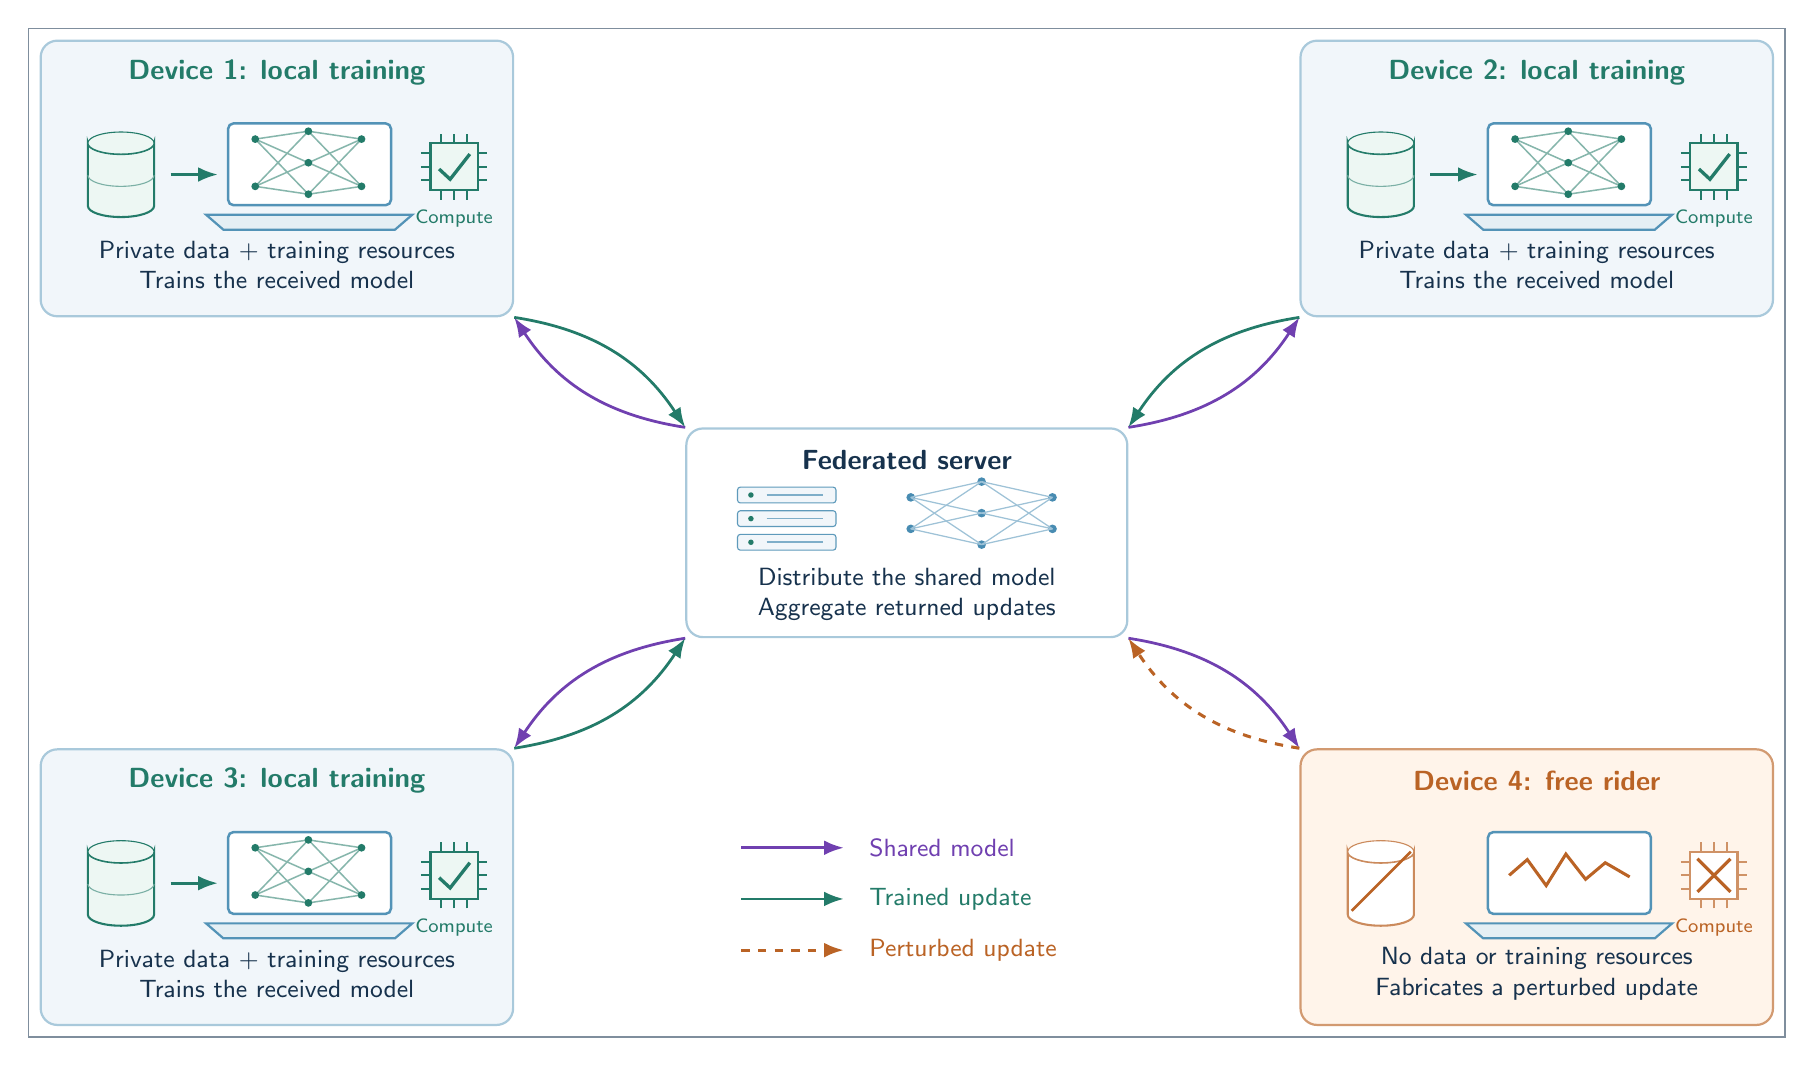
\begin{tikzpicture}[
 font=\sffamily\small,text=ink,
 card/.style={draw=blue!40,fill=pale,rounded corners=6pt,
  minimum width=6cm,minimum height=3.5cm,line width=.8pt},
 download/.style={-{Latex[length=2.5mm]},draw=sharedmodel,line width=1pt},
 trained/.style={-{Latex[length=2.5mm]},draw=green,line width=1pt},
 fabricated/.style={-{Latex[length=2.5mm]},draw=orange,line width=1.1pt,dashed},
 linklabel/.style={font=\sffamily\scriptsize,fill=white,inner sep=3pt,sloped}
 ]

% Local behavior is illustrative; the server does not observe local telemetry.
\node[card,minimum width=5.6cm,minimum height=2.65cm,fill=white] (server) at (0,0) {};
\node[font=\sffamily\bfseries\normalsize] at (0,.93) {Federated server};
\foreach \y in {-.12,.18,.48} {
 \draw[draw=blue!75,fill=pale,rounded corners=1pt] (-2.15,\y-.1) rectangle (-.9,\y+.1);
 \fill[green] (-1.98,\y) circle (.035);
 \draw[blue!60,line width=.6pt] (-1.78,\y) -- (-1.06,\y);
}
\foreach \x/\y in {.05/.45,.05/.05,.95/.65,.95/.25,.95/-.15,1.85/.45,1.85/.05} {
 \fill[blue!85] (\x,\y) circle (.055);
}
\foreach \a in {.45,.05} {\foreach \b in {.65,.25,-.15} {
 \draw[blue!45,line width=.45pt] (.05,\a)--(.95,\b);
}}
\foreach \a in {.65,.25,-.15} {\foreach \b in {.45,.05} {
 \draw[blue!45,line width=.45pt] (.95,\a)--(1.85,\b);
}}
\node[align=center] at (0,-.78) {Distribute the shared model\\Aggregate returned updates};

\foreach \x/\y/\id in {-8/4.5/1,8/4.5/2,-8/-4.5/3} {
 \begin{scope}[shift={(\x,\y)}]
  \node[card] (device\id) at (0,0) {};
  \node[font=\sffamily\bfseries\normalsize,text=green] at (0,1.35) {Device \id: local training};
  % Private local dataset.
  \draw[draw=green,fill=greenpale,line width=.75pt] (-2.4,-.35) -- (-2.4,.45)
   arc[start angle=180,end angle=360,x radius=.42,y radius=.14]
   -- (-1.56,-.35) arc[start angle=0,end angle=-180,x radius=.42,y radius=.14];
  \draw[draw=green,fill=greenpale] (-1.98,.45) ellipse[x radius=.42,y radius=.14];
  \draw[green!60] (-2.4,.04) arc[start angle=180,end angle=360,x radius=.42,y radius=.14];
  \draw[trained] (-1.35,.05) -- (-.75,.05);
  % Laptop with a compact model icon.
  \draw[draw=blue!80,fill=white,rounded corners=2pt,line width=.9pt] (-.62,-.34) rectangle (1.45,.7);
  \draw[draw=blue!80,fill=blue!12,line width=.8pt] (-.9,-.46) -- (1.72,-.46)
   -- (1.5,-.65) -- (-.68,-.65) -- cycle;
  \begin{scope}[shift={(.4,.2)},x=1.5cm,y=1cm]
   \foreach \a in {-.3,.3} { \foreach \b in {-.4,0,.4} {
    \draw[green!55,line width=.55pt] (-.45,\a)--(0,\b);
    \draw[green!55,line width=.55pt] (0,\b)--(.45,\a);
   }}
   \foreach \nx/\ny in {-.45/-.3,-.45/.3,0/-.4,0/0,0/.4,.45/-.3,.45/.3}
    \fill[green] (\nx,\ny) circle[radius=1.4pt];
  \end{scope}
  % Available training compute, shown as a processor with a check mark.
  \draw[green,fill=greenpale,line width=.8pt] (1.95,-.15) rectangle (2.55,.45);
  \foreach \pin in {-.02,.15,.32} {
   \draw[green,line width=.7pt] (1.83,\pin)--(1.95,\pin);
   \draw[green,line width=.7pt] (2.55,\pin)--(2.67,\pin);
  }
  \foreach \pin in {2.08,2.25,2.42} {
   \draw[green,line width=.7pt] (\pin,-.27)--(\pin,-.15);
   \draw[green,line width=.7pt] (\pin,.45)--(\pin,.57);
  }
  \draw[green,line width=1.2pt] (2.06,.12)--(2.2,-.01)--(2.45,.31);
  \node[font=\sffamily\scriptsize,text=green] at (2.25,-.51) {Compute};
  \node[align=center] at (0,-1.1) {Private data + training resources\\Trains the received model};
 \end{scope}
}

\begin{scope}[shift={(8,-4.5)}]
 \node[card,draw=orange!65,fill=orangepale] (rider) at (0,0) {};
 \node[font=\sffamily\bfseries\normalsize,text=orange] at (0,1.35) {Device 4: free rider};
 % Crossed data and compute symbols show unavailable training resources.
 \draw[draw=orange!75,fill=white,line width=.75pt] (-2.4,-.35) -- (-2.4,.45)
  arc[start angle=180,end angle=360,x radius=.42,y radius=.14]
  -- (-1.56,-.35) arc[start angle=0,end angle=-180,x radius=.42,y radius=.14];
 \draw[draw=orange!75,fill=white] (-1.98,.45) ellipse[x radius=.42,y radius=.14];
 \draw[orange,line width=1pt] (-2.35,-.3)--(-1.6,.45);
 \draw[orange!70,fill=white,line width=.8pt] (1.95,-.15) rectangle (2.55,.45);
 \foreach \pin in {-.02,.15,.32} {
  \draw[orange!70,line width=.7pt] (1.83,\pin)--(1.95,\pin);
  \draw[orange!70,line width=.7pt] (2.55,\pin)--(2.67,\pin);
 }
 \foreach \pin in {2.08,2.25,2.42} {
  \draw[orange!70,line width=.7pt] (\pin,-.27)--(\pin,-.15);
  \draw[orange!70,line width=.7pt] (\pin,.45)--(\pin,.57);
 }
 \draw[orange,line width=1.15pt] (2.04,-.06)--(2.46,.36);
 \draw[orange,line width=1.15pt] (2.04,.36)--(2.46,-.06);
 \node[font=\sffamily\scriptsize,text=orange] at (2.25,-.51) {Compute};
 \draw[draw=blue!80,fill=white,rounded corners=2pt,line width=.9pt] (-.62,-.34) rectangle (1.45,.7);
 \draw[draw=blue!80,fill=blue!12,line width=.8pt] (-.9,-.46) -- (1.72,-.46)
  -- (1.5,-.65) -- (-.68,-.65) -- cycle;
 \draw[orange,line width=1.1pt] (-.35,.15)--(-.12,.35)--(.12,.02)
  --(.37,.42)--(.62,.1)--(.87,.31)--(1.18,.13);
 \node[align=center] at (0,-1.1) {No data or training resources\\Fabricates a perturbed update};
\end{scope}

\draw[download] (server.north west) to[bend left=24] (device1.south east);
\draw[trained] (device1.south east) to[bend left=24] (server.north west);
\draw[download] (server.north east) to[bend right=24] (device2.south west);
\draw[trained] (device2.south west) to[bend right=24] (server.north east);
\draw[download] (server.south west) to[bend right=24] (device3.north east);
\draw[trained] (device3.north east) to[bend right=24] (server.south west);
\draw[download] (server.south east) to[bend left=24] (rider.north west);
\draw[fabricated] (rider.north west) to[bend left=24] (server.south east);
\draw[download] (-2.1,-4.0) -- (-.8,-4.0);
\node[anchor=west,text=sharedmodel] at (-.6,-4.0) {Shared model};
\draw[trained] (-2.1,-4.65) -- (-.8,-4.65);
\node[anchor=west,text=green] at (-.6,-4.65) {Trained update};
\draw[fabricated] (-2.1,-5.3) -- (-.8,-5.3);
\node[anchor=west,text=orange] at (-.6,-5.3) {Perturbed update};
\begin{scope}[on background layer]
 \draw[ink!55,line width=.6pt]
  ([xshift=-4pt,yshift=-4pt]current bounding box.south west)
  rectangle ([xshift=4pt,yshift=4pt]current bounding box.north east);
\end{scope}
\end{tikzpicture}
\end{document}
